%% USPSC-Introducao.tex

% ----------------------------------------------------------
% Introdução (exemplo de capítulo sem numeração, mas presente no Sumário)
% ----------------------------------------------------------
\chapter[Introduction]{Introduction}
\label{Introduction}

% In 1985, the first interaction between medicine and robotics occurred with the \textit{PUMA} manipulator, which was used for brain biopsies. At the end of the 20th century, there was a fundamental transformation in the methods used to perform surgical procedures. For many interventions, the invasive nature has been considerably reduced, bringing superior results such as better survival rates, lower incidence of complications, and faster recovery in terms of functional health and quality of life \cite{yoon2023robotic}.

% Surgical interventions further expanded with the introduction of the \textit{da Vinci} robot in 2000, which enabled tasks to be performed with precision and strength beyond human capability. The \textit{da Vinci} system marked a significant advancement in minimally invasive surgery (MIS) - a set of surgical techniques that minimize the size and number of incisions required, thereby reducing patient trauma, recovery time, and risk of complications \cite{morrell2021history}. The success of MIS, facilitated by robotic assistance, has driven intensive research and development of new surgical robots in recent years \cite{minimal}.

% spine robots intro? types of robots? collaborative robots?
In cranial neurosurgery, intracranial electrode placement is a core procedure for both diagnostic and therapeutic purposes, particularly in the management of epilepsy and movement disorders. These procedures require the accurate insertion of electrodes into specific brain regions, reason why robotic assistance is increasingly utilized. Among the most common applications are stereoelectroencephalography (SEEG) for epilepsy diagnosis and deep brain stimulation (DBS) for treating movement disorders such as Parkinson's disease \cite{kim2021contemporaneous}.

SEEG involves the implantation of multiple depth electrodes into targeted brain areas to localize epileptogenic zones that are responsible for seizure generation. This technique provides critical information for surgical planning in drug-resistant epilepsy cases. In contrast, DBS is a therapeutic intervention where electrodes are implanted into subcortical structures, such as the subthalamic nucleus or globus pallidus, to deliver electrical stimulation that modulates abnormal neural circuits. DBS has become a standard treatment for movement disorders, notably Parkinson's disease, essential tremor, and dystonia, offering significant improvements in motor symptoms and quality of life for affected patients \cite{liu2020frameless}.

Robotic systems are increasingly being adopted for intracranial electrode implantation by maintaining accuracy and enhancing surgical workflow. Neuromate, introduced in the late 1990s, was among the first dedicated robotic platforms for neurosurgery, enabling automated and precise placement of electrodes for procedures such as SEEG and DBS. The subsequent development of ROSA brought further advancements, expanding its applications to include spine surgery and other orthopedic interventions. In epilepsy surgery, robotic assistance has proven particularly valuable, offering similar accuracy in localizing and targeting epileptogenic zones comparable to traditional methods, while significantly reducing operative time \cite{kaewborisutsakul2024usefulness}.

Although SEEG requires precise electrode placement, its accuracy requirements are generally less stringent than those for deep brain stimulation (DBS), which demands submillimeter precision due to the need for targeting specific anatomical nuclei. SEEG, in contrast, is hypothesis-driven and aims to sample broader brain regions based on clinical hypotheses rather than discrete anatomical targets \cite{bonda2021robot}.

SEEG represents a clinically relevant and technically feasible entry point for robotic intervention, given its procedural characteristics and the growing demand for minimally invasive, accurate, and efficient electrode implantation in epilepsy surgery. Accordingly, this work focuses on the evaluation of a collaborative robotic system designed for SEEG electrode placement called \textit{Yara}, as an initial and essential step toward advancing robotic assistance in intracranial procedures. To contextualize this objective, the following chapters review the clinical aspects of epilepsy (Sec. \ref{sec:epi}), the classification and impact of seizure types, and the current therapeutic strategies available (Sec. \ref{sec:methods}).

\chapter[Objectives]{Objectives}
\label{Objectives}

The primary objective of this work is to evaluate the accuracy of the Yara collaborative robotic platform for intracranial electrode placement during SEEG (stereoelectroencephalography) procedures. This evaluation is performed using anatomical phantoms that closely mimic human cranial structures, enabling measurement of electrode placement accuracy. By focusing on phantom-based experiments, the study aims to establish a baseline for the system’s technical performance in a controlled environment, prior to any clinical application.

A key objective is the design and fabrication of cranial phantoms specifically for SEEG accuracy validation. These phantoms are developed to replicate the anatomical and mechanical properties of the human skull and brain, allowing for reproducible assessment of electrode placement. The creation of these phantoms is essential to ensure that the experimental conditions closely simulate those encountered in actual surgical scenarios.

Finally, the study aims to conduct accuracy validation tests using the Yara robotic platform, both in the laboratory and in the operating room environment. By performing electrode placement trials in these settings, the work seeks to assess the system’s performance under different conditions, identify potential sources of error, and provide quantitative data on placement accuracy.

\chapter[Literature Review]{Literature Review}
\label{Literature}

\section{Epilepsy}\label{sec:epi}

% @gui one for what is epilepsy
%...
Epilepsy is a chronic brain disease characterized by a long-lasting predisposition to generate seizures, not caused by any immediate insult to the central nervous system, and by the neurobiological, cognitive, psychological, and social consequences of recurrent seizures \cite{beghi2020epidemiology}. This is the most common neurological disease worldwide, affecting different social classes, ages, and geographic locations \cite{ngugi2010estimation}.

% what is epilepsy seizures
The definition of epileptic seizures is: repeated and transient episodes that manifest themselves through patterned behaviors, mirroring the underlying neural processes associated with the condition \cite{fisher2005epileptic}. Although all people with epilepsy experience seizures, not all individuals with seizures have epilepsy. Epileptic seizures can also occur after an acute injury to the central nervous system (CNS) of structural, systemic, toxic, or metabolic origin. These events are considered acute manifestations of the insult and may not occur when the underlying cause has been removed or the acute phase has passed \cite{beghi2010recommendation}.

% types of epilepsy seizures
Epileptic seizures are categorized according to three main characteristics: origin in the brain, state of consciousness during the seizure, and level of body movement. Seizures can be classified as focal or generalized based on the first characteristic. The second characteristic considers whether consciousness is intact or impaired during the seizure, while the third characteristic refers to body movement, which may present motor or non-motor reactions \cite{beghi2020epidemiology}.

Motor seizures encompass a variety of distinct manifestations. Atonic crises are characterized by a sudden and temporary loss of muscle tone, resulting in a sudden fall of the individual. On the other hand, tonic crises involve a sudden and prolonged increase in muscle tone, leading to intense stiffness. Clonic seizures are marked by rhythmic and repetitive muscle contractions, which can affect different parts of the body, while myoclonic seizures are characterized by rapid and sudden muscle contractions that can involve a specific muscle group or the entire body. Epileptic spasms, automatisms, and hyperkinetic seizures are also categorized \cite{sarmast2020current}.

On the other hand, non-motor crises can present different forms of manifestation. They can be autonomic, involving dysfunctions in the autonomic nervous system, such as changes in blood pressure or heart rate. In addition, there may be crises of behavioral arrest, during which the individual may appear paralyzed or unable to perform voluntary movements. Cognitive crises affect cognitive function and may include memory lapses or mental confusion. Emotional crises are related to changes in the emotional state, such as feelings of fear, anxiety, or euphoria. Finally, sensory crises affect the senses and can cause abnormal sensations, such as visual or auditory hallucinations \cite{sarmast2020current}.

\section{Treatment Methods} \label{sec:methods}

% @gui one for what are the treatments
%...
Among patients with epilepsy, approximately 40\% experience drug-resistant seizures, representing a significant portion of the global population estimated at 70 million people. In such cases, surgery may be considered as a therapeutic option. This procedure is indicated for patients with disabling focal epilepsy who are unresponsive to drug treatment and whose seizures originate in a specific region of the brain that can be removed with minimal risk of neurological or cognitive dysfunction \cite{miller2013surgical}. Surgery offers the possibility of significantly improving the quality of life of these patients, providing adequate control of seizures and reducing dependence on high-cost and potentially harmful antiepileptic medications.

Correctly locating the focus of seizures is a crucial aspect in preparing for surgery in patients with epilepsy \cite{miller2013surgical}. Localization methods are applied to accurately determine the focal region, aiming to minimize the invasiveness of the surgery while seeking complete removal of the area of focus to cease seizures. Accuracy in locating the focus has a significant impact on the effectiveness of the surgical procedure, as it can help avoid undesirable consequences associated with the resection of unaffected areas.

This is especially important, as the removal of critical areas of the brain can result in functional deficits, such as impairment of speech, memory, motor coordination, among other functions, depending on the location of the focus. Therefore, ensuring accurate location of the focus is essential to guarantee good surgical results and minimize potential adverse effects.

\subsection{Video-EEG} \label{sec:non-invasive-eeg}

% @gui EEG
%...
Before progressing to invasive procedures, a non-invasive analysis is typically performed to identify potential areas of seizure foci and to guide further investigation. Scalp EEG is the primary non-invasive technique used for this purpose. Electrodes are placed on the patient's scalp using a cap or similar device, enabling monitoring during interictal (between seizures), ictal (during seizures), and post-ictal (after seizures) periods. This superficial electrode arrangement measures electrical potentials generated by neuronal activity near the skull. Standard systems use 32, 64, or 96 electrodes distributed across the scalp, with higher-density arrays (up to 256 channels) available for more detailed studies \cite{Sun2023}. Scalp EEG is essential for initial diagnosis and localization of seizure activity, providing critical information before invasive methods are considered \cite{miller2013surgical}.

\subsection{Invasive EEG: Subdural EEG (SDE) and Stereoencephalography (SEEG)}

%@gui subdural EEG
%...
Subdural EEG (SDE), also known as electrocorticography (ECoG), was developed to provide more precise measurement of brain activity than scalp EEG. In SDE, an electrode array is placed directly on the surface of the cortex after a portion of the skull is removed, as illustrated in Fig. \ref{fig:eeg-ecog-seeg}. This direct contact enables the acquisition of signals with higher fidelity and less noise compared to scalp EEG \cite{lesser2010subdural}. The electrodes typically remain in place for several days to record both ictal and interictal activity. However, SDE is highly invasive, requiring two craniotomies, one for electrode placement and another for removal, and carries a significant risk of postoperative infection, often related to surgical contamination. These drawbacks have motivated the development of alternative methods, such as SEEG, which aim to reduce invasiveness and associated complications \cite{jehi2021comparative}.

% @gui SEEG
%...
In France, in the 1950s, Jean Tailarach and Jean Bancaud developed a method that aims to monitor deep parts of the cortex through the insertion of deep electrodes, seeking to replace the SDE \cite{mazoyer2008memoriam}. This method was called Stereoelectroencephalography (SEEG) and today it is one of the most adopted invasive methods for locating the focal zone of seizures. SEEG does not present many of the problems presented by SDE. In this method, cylindrical electrodes (more like small wires) are introduced through small holes in the skull, without the need for craniotomy. SEEG has lower rates of infection, hemorrhage, neurological deficits, and morbidity compared to SDE, in addition to being a faster procedure, allowing the analysis of deeper brain tissues and having shown greater effectiveness in localizing and controlling seizures after surgical treatment \cite{fiani2021stereoelectroencephalography}. Fig. \ref{fig:eeg-ecog-seeg} illustrates the positioning of electrodes in scalp EEG, Subdural EEG (electrocorticography), and SEEG.

% fig scalp eeg, ecog and seeg
\begin{figure}
     \centering
     \includegraphics[width=0.99\textwidth]{USPSC-img/eeg-ecog-seeg.png}
     \caption{Positioning of electrodes in scalp electroencephalography, electrocorticography, and stereoelectroencephalography procedures respectively \cite{shen2020ml} \cite{blausen2014medical} \cite{Jones2018}.}
     \label{fig:eeg-ecog-seeg}
\end{figure}

% Metrics for analyzing the accuracy
%...euclidean distance and etc
Electrodes implanted during SEEG are used to properly identify the epileptogenic zone (EZ) \cite{Jones2018}. Planning prior to surgery is carried out to define the number of electrodes, the position of the entry points, and the target point of each electrode. Metrics are defined for evaluating the position of the SEEG implants. Entry points are defined as the point at which the electrode initiates contact with the surface of the brain or the skull. Target points are defined as the final position of the electrode, usually in a region within the brain.

Widely adopted metrics for evaluating the accuracy of the electrode placement are the Euclidean distance between the planned entry points and the post-surgical entry points, and the distance between the planned target points and the post-surgical target points.

\section{Stereoelectroencephalography: Operation Methods} \label{sec:seeg-methods}

% classic methods of SEEG
% Stereotactic Arc...
% Tailarach
%...
\subsection{Stereotaxy}

SEEG operation techniques began in the 1950s with Jean Talairach and Jean Bancaud, who developed x‑ray–based methods for planning and verifying electrode positioning. Since then the development of mechanical  stereotactic apparatus to fix the skull and guide electrode placement concentrated in the mid‑20th century (late 1940s–1950s). The early Tailarach apparatus featured skull‑fixation pins, a support for the x‑ray tube, and radiographic film \cite{mazoyer2008memoriam}. Contemporary popular frames, such as the Leksell frame developed in Sweden around the same period, trace their origins to these innovations.

With the advent of computed tomography, surgeries began to be planned based on slices, allowing a three-dimensional understanding of the areas of investigation. Devices that use the three-dimensionality of tomography images were adapted, adding a support with a diagonal cut in the shape of an N, allowing the calculation of the height of each tomography slice in relation to the device coordinates. This system became known as the N-Localizer and is widely used in current neurosurgeries \cite{lozano2009textbook}.

\begin{figure}[h]
     \centering
     \begin{subfigure}{0.69\textwidth}
          \includegraphics[width=\linewidth]{USPSC-img/tailarach-frame.jpg}
          \caption{}
     \end{subfigure}\hfill
     \begin{subfigure}{0.29\textwidth}
          \includegraphics[width=\linewidth]{USPSC-img/tailarach-coordinates.jpeg}
          \caption{}
     \end{subfigure}
     \caption{(a) presents Tailarach's \textit{frame} with x-ray supports and (b) presents an example x-ray image alongside the coordinate system developed by Tailarach \cite{mazoyer2008memoriam}.}
     \label{fig:tailarach-frame}
\end{figure}

\subsection{Frame-based Surgeries} \label{sec:stereotactics}

The earliest SEEG technique involved introducing electrodes in parallel trajectories, normal to the sagittal view, using the Cartesian map called Talairach coordinates \cite{mazoyer2008memoriam}. Subsequently, variations of the technique were explored with the introduction of  stereotactic arcs that can be fixed to devices such as the Leksell or CRW and that allow the introduction of oblique electrodes. Therefore, the assessment of the impact on precision between different techniques for implanting oblique or orthogonal electrodes was studied in \cite{Iordanou2019}. Figure \ref{fig:leksell} presents the Leksell G apparatus and the N-Localizer.

Originally, the calculation of the coordinates of each electrode in relation to the apparatus was carried out manually, using the N-Localizer geometry. Some softwares for surgical planning were developed so that the calculation of the coordinates of the entry and target points was automated using image processing methods containing the N-Localizer \cite{dasgupta2022previous}. These softwares also features planning tools, such as fusing standard CT images and MRI images.

% fig leksell
\begin{figure}[h]
     \centering
     \includegraphics[width=0.7\textwidth]{USPSC-img/leksell.png}
     \caption{Frame Leksell G without N-Localizer and with N-Localizer respectively \cite{rojas2016eval}.}
     \label{fig:leksell}
\end{figure}

Image fusion allows precise surgical planning by combining preoperative MRI to assess vascular structures and functional anatomy near electrode trajectories and intraoperative CT to permit frame positioning. During surgery, a stereotactic frame and N-Localizer are attached to the patient's head, followed by an intraoperative CT scan. This scan is fused with the preoperative MRI, enabling the planning software to identify N-Localizer fiducials and accurately compute coordinates for electrode placement. These coordinates are then inputted into the stereotactic frame or arc, guiding the surgeon in positioning each electrode along the planned trajectory.

%In this regard, Medtronic, with the Stealth Autoguide \cite{medtronic}, developed a system that allows the tool to be fixed, facilitating the drilling of the skull and the fixation of the guide screw.

Surgeries based on stereotactic devices have a broad history of use, but they also have disadvantages in relation to more recent systems, such as robotic systems. Among the disadvantages, the  stereotactic frames operation requires the placement of the apparatus at the beginning of the surgery, followed by a CT generally located in another room, and the fusion of this CT to the MRI taken used for planning. This process is necessary to calculate the coordinates of each entry point and target in relation to the frame. This CT scan during surgery is not necessary with the use of robotic systems in surgeries called frameless.

\begin{table}[!h]
     \centering
     \caption{Comparison between frame-based and \textit{frameless} procedures for SEEG.}
     \label{tab:frame-vs-frameless}
     \begin{tabular}{p{0.95\linewidth}}

          \textbf{Frame-based surgery}                          \\
          \toprule
          1. Preoperative imaging (MRI, EEG) and clinical evaluation

          2. Trajectory planning based on preliminary evidence before surgery

          3. Start of surgery and fixation of the head in the stereotactic apparatus

          4. Tomography with stereotactic frame and N-Localizer

          5. Fusion of MRI and intraop CT with frame to calculate the coordinates of each electrode in relation to the apparatus

          6. Using the  stereotactic ruler, drill the skin and skull using a 3 mm drill with an appropriate end point

          7. Fixing a guide screw to the skull, to serve as a guide for electrode insertion

          8. Using the guide screw, insert the temporary stylet into the intracranial space to the target point for electrode guidance

          9. Remove the temporary stylet and, through the guide screw, insert the depth electrode into the intracranial space to the predefined destination

          10. Screw the electrode cover onto the guide screw

          11. Repeat steps 6 to 10 for the remaining electrodes \\
          \bottomrule
          \\

          \textbf{Robot-assisted frameless surgery}             \\
          \toprule
          1. MRI, EEG, and preliminary surgery exams, as well as assessment of patient symptoms

          2. Planning trajectories based on preliminary evidence before surgery using the robot's interface

          3. Facial registration using fiducial points of the face

          4. Positioning the robot and drilling the skin and skull using a 3 mm drill with an appropriate limit stroke

          5. Fixing the guide screw to the skull

          6. Using the guide screw, insert the temporary stylet into the intracranial space to the target point for electrode guidance

          7. Remove the temporary stylet and, through the guide screw, insert the depth electrode into the intracranial space to the predefined destination

          8. Screw the electrode cover onto the guide screw

          9. Repeat steps 4 to 8 for the remaining electrodes   \\
          \bottomrule
     \end{tabular}
\end{table}

The Table \ref{tab:frame-vs-frameless} presents a comparison between the procedures necessary to perform frame-based surgery compared to frameless surgeries. The greater number of steps during surgery increases the time needed to perform the surgery and may result in loss of accuracy due to non-deterministic procedures and possible human errors.

Performing a CT scan during surgery is time-consuming. The frame-based process requires a tomography with the stereotactic device immediately after its placement. While having a CT scanner available in the same operating room would streamline logistics, this setup is rarely feasible, as most hospitals do not have a dedicated CT scanner for each operating room. Although some facilities offer operating rooms equipped with CT scanners, their limited availability and competition with other ongoing surgeries complicate scheduling and scalability. As a result, the typical solution is to transport the sedated patient to a separate CT scanner, which increases surgery time and possibly introduces additional risks.

Another significant source of error arises from the fusion of intraoperative CT images acquired with the stereotactic device and preoperative MRI images. Image fusion involves the precise alignment of two volumetric datasets - typically, the CT and MRI scans - so that both accurately represent the same anatomical structures. This process is necessary because the spatial orientation and coordinate systems of the CT and MRI volumes differ in space due to variations in patient positioning and scanner-specific parameters. Imperfect alignment during fusion can introduce discrepancies in the localization of entry and target points, thereby contributing to the overall error in electrode placement.

The alignment of the preoperative MRI with the intraoperative CT, in the case of SEEG surgery, allows the planning performed on the MRI to be accurately transferred to the CT acquired with the  stereotactic apparatus. In this way, the result of the fusion is the planning of the surgery, containing entry and target points in the same reference as the apparatus images, thus allowing the calculation of the coordinates necessary to align the ruler or  stereotactic arc in each trajectory. Even in the most ideal case, this process is not perfect and will contribute to the final error of each trajectory. In summary, the steps of fixing the device, transporting the patient to the CT scanner, and performing image fusion are significant sources of both surgical errors and increased operative time in procedures based on stereotactic devices.

\subsection{Robot-based Surgeries}

\begin{figure}
     \centering
     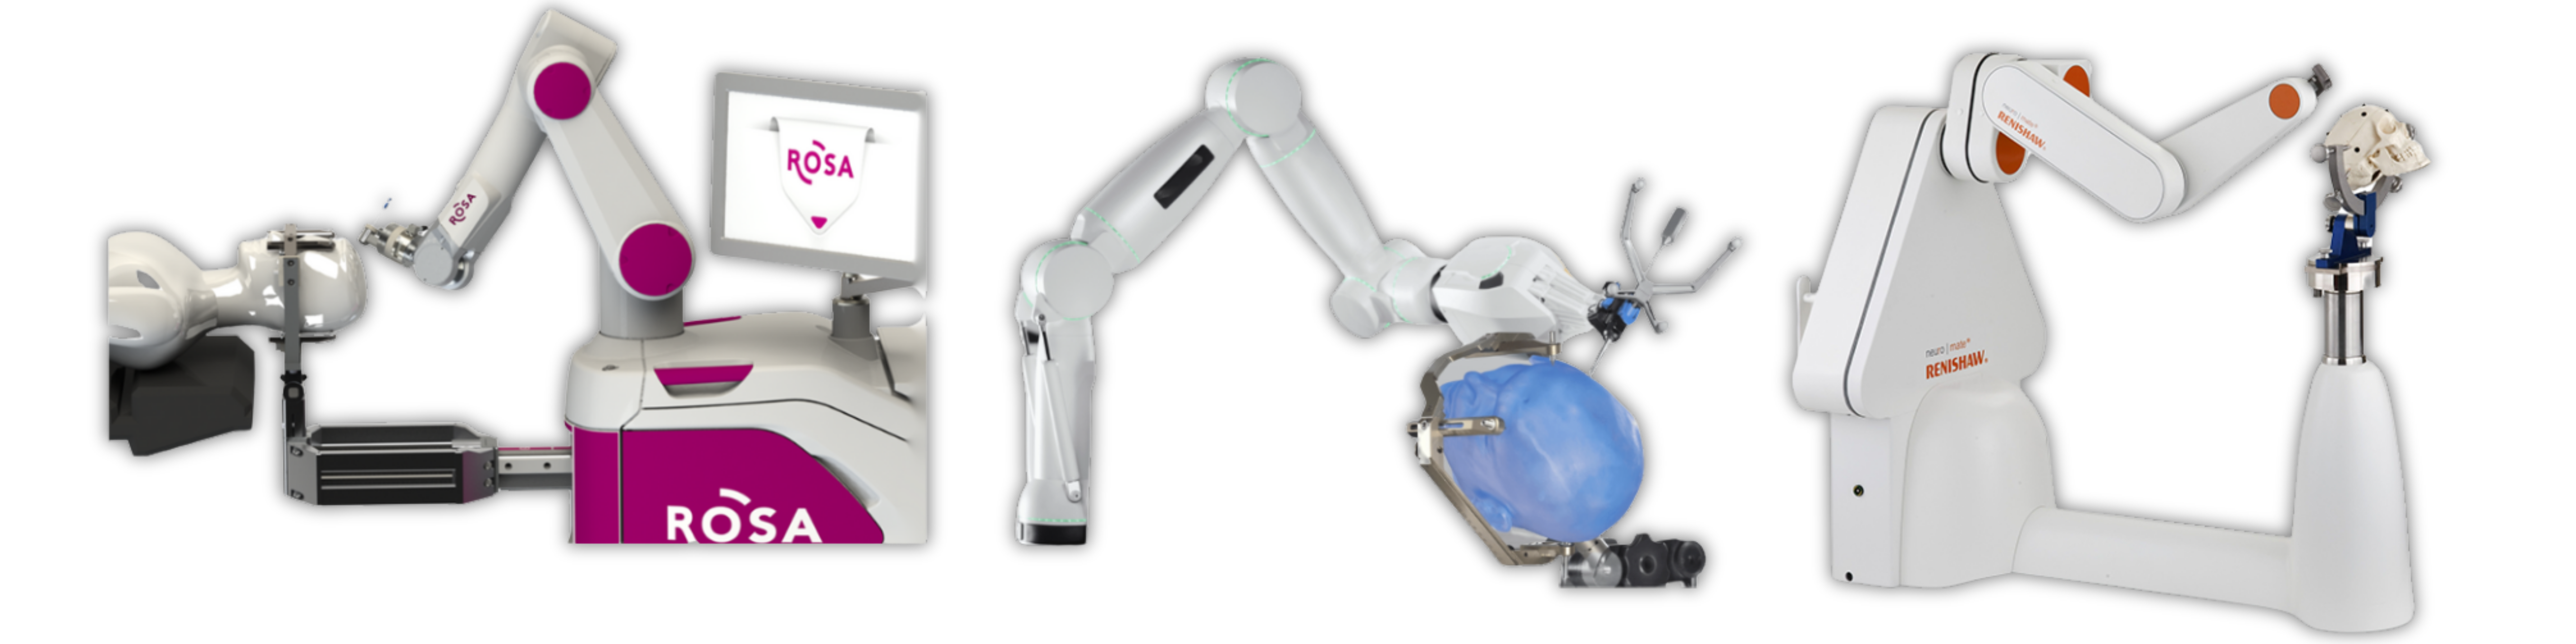
\includegraphics[width=0.99\textwidth]{USPSC-img/robots_enhanced.png}
     \caption{Robots capable of performing SEEG surgeries: Zimmer Biomet ROSA ONE Brain, Brainlab Cirq and Renishaw Neuromate respectively.}
     \label{fig:robots}
\end{figure}

There are studies in the literature that highlight the development of \textit{frameless} robotic systems for SEEG surgeries, aiming to improve surgical workflow, accuracy, and safety \cite{gonzalez2016technique, cardinale2013stereoelectroencephalography}. Most of the technical details and innovations in these systems are published as patents rather than in peer-reviewed scientific articles, mainly because of the commercial interests involved.

Renishaw's Neuromate, introduced in 1998, was the first commercially available robot for SEEG neurosurgery \cite{cardinale2013stereoelectroencephalography}. Fig. \ref{fig:robots} shows Neuromate, which features a triangular base and supports for skull fixation using Mayfield or Leksell frames. Subsequently, Medtech (acquired by Zimmer Biomet) developed ROSA ONE Brain, and Brainlab introduced Cirq, both capable of performing SEEG procedures. These systems also support other neurosurgical interventions, including brain biopsies and deep brain stimulation (DBS) for conditions such as Parkinson's disease.

% neuromate
Neuromate was the first commercially available robot for neurosurgery, but its adoption faces significant limitations. A major constraint is the requirement for a dedicated operating room, as the system is not designed for mobility between rooms. This complicates hospital logistics and often prevents acquisition due to infrastructure demands. Additionally, Neuromate features only 5 degrees of freedom (DOF), making it an under-actuated system with reduced mobility and positioning capabilities compared to conventional 6-DOF robotic platforms \cite{kajita2015installation}.

% cirq
% The Cirq robotic system is used with a full neuronavigation system. A device with reflective spheres is fixed to the robot's flange. This device is viewed by an infrared stereo camera and the position of the tool is calculated. Its adjustment is done semi-automatically, where the surgeon approaches the robot to the desired position and the robot adjusts itself with an actuator fixed to its flange. The neuronavigator is used to operate this system, which has: a camera carriage; a screen carriage; and a robotic manipulator fixed to the operating table. Combined with other devices present in the operating room, these three devices bring difficulties in logistics and in organizing the space in the room compared to systems that have only one carriage.

ROSA ONE Brain is not collaborative. In other words, even though it is designed to perform a task together with the surgeon, ROSA does not feature sensors that are present in collaborative systems, such as measuring joint torque, and collision detection with automatic braking. This aspect makes ROSA a conventional robot applied to collaborative tasks, putting doctor and patient higher risk level compared to collaborative systems. Yara, the system proposed in this project, integrates collaborative robots, validated worldwide for tasks that involve joint operations with humans, ensuring the surgeon's and patient's safety.

Typically, non-collaborative industrial robots are required to operate at a safe distance from humans according to workplace safety regulations, but surgical robots are not subject to these industrial standards. Current commercial neurosurgical systems do not incorporate collaborative robotics technology. KUKA pioneered the introduction of collaborative robots for medical applications with the KUKA LBR Med, which is certified according to international medical safety standards. Collaborative systems like these enhance safety during robotic manipulation in surgery, offering advantages over existing non-collaborative platforms.

% The Stealth AutoGuide by Medtronic \cite{medtronic} is a compact robotic system that attaches directly to the Mayfield head clamp, rather than functioning as a full robotic arm. It assists the surgeon by aligning the trajectory of each electrode during SEEG procedures. The system operates in conjunction with their neuronavigation platform, which is widely used for image-guided surgery. Neuronavigation systems typically employ either optical (stereo camera) or electromagnetic tracking to display instrument positions relative to the patient's anatomy, using preoperative CT or MRI data to guide access to specific brain targets. By integrating with these systems, the small robot arm improves the accuracy of electrode placement, providing precise guidance along planned trajectories.


Yara is a collaborative robotic platform developed for frameless intracranial electrode placement procedures, designed to offer accuracy, reduced surgical time, and enhanced safety compared to traditional frame-based methods. The system integrates planning software for defining electrode entry and target points, MRI/CT image fusion, automated patient registration using depth cameras, and collision-free robotic positioning. In this work, we present a comprehensive evaluation of the accuracy of the Yara platform for SEEG electrode placement, based on phantom experiments that simulate clinical conditions.

% %%%%%%%%%%%